\documentclass[tikz]{standalone}

\usepackage{tikz}
\usepackage{pagecolor}
\usepackage{color}
\usepackage{blkarray}

\definecolor{mygray}{gray}{0.7}
\pagecolor{white}

\begin{document}
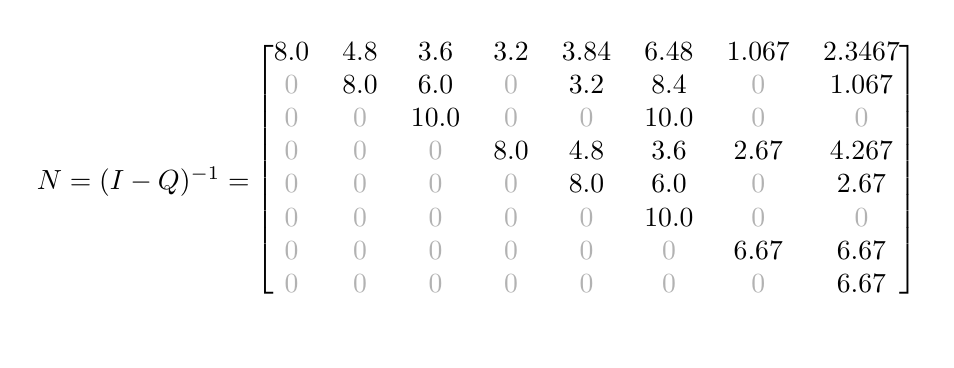
\begin{tikzpicture}

\node (0) [] at (0, 0) {$N = (I - Q)^{-1} =
\begin{blockarray}{[cccccccccc]}
    8.0 & 4.8 & 3.6 & 3.2 & 3.84 & 6.48 & 1.067 & 2.3467 \\
    \textcolor{mygray}{0} & 8.0 & 6.0 & \textcolor{mygray}{0} & 3.2 & 8.4 & \textcolor{mygray}{0} & 1.067 \\
    \textcolor{mygray}{0} & \textcolor{mygray}{0} & 10.0 & \textcolor{mygray}{0} & \textcolor{mygray}{0} & 10.0 & \textcolor{mygray}{0} & \textcolor{mygray}{0}  \\
    \textcolor{mygray}{0} & \textcolor{mygray}{0} & \textcolor{mygray}{0} & 8.0 & 4.8 & 3.6 & 2.67 & 4.267 \\
    \textcolor{mygray}{0} & \textcolor{mygray}{0} & \textcolor{mygray}{0} & \textcolor{mygray}{0} & 8.0 & 6.0 & \textcolor{mygray}{0} & 2.67 \\
    \textcolor{mygray}{0} & \textcolor{mygray}{0} & \textcolor{mygray}{0} & \textcolor{mygray}{0} & \textcolor{mygray}{0} & 10.0 & \textcolor{mygray}{0} & \textcolor{mygray}{0} \\
    \textcolor{mygray}{0} & \textcolor{mygray}{0} & \textcolor{mygray}{0} & \textcolor{mygray}{0} & \textcolor{mygray}{0} & \textcolor{mygray}{0} & 6.67 & 6.67 \\
    \textcolor{mygray}{0} & \textcolor{mygray}{0} & \textcolor{mygray}{0} & \textcolor{mygray}{0} & \textcolor{mygray}{0} & \textcolor{mygray}{0} & \textcolor{mygray}{0} & 6.67 \\
\end{blockarray}
$};
\end{tikzpicture}
\end{document}
